\documentclass{report}
\usepackage[utf8]{inputenc}
\usepackage[top=1cm, bottom=2cm, left=2cm, right=2cm]{geometry}
\usepackage[francais]{babel}
\usepackage[T1]{fontenc}
\usepackage{graphicx}
\usepackage{subcaption}
\usepackage{listings}
\usepackage{hyperref}
\usepackage{wrapfig}

\title{Rapport}
\author{François PIAT}
\date{WEEK 7}

\begin{document}

\maketitle

\chapter*{Profiling}
Performances de resample-image avec TBB: 
\begin{figure}[h!]
	\begin{flushleft}
		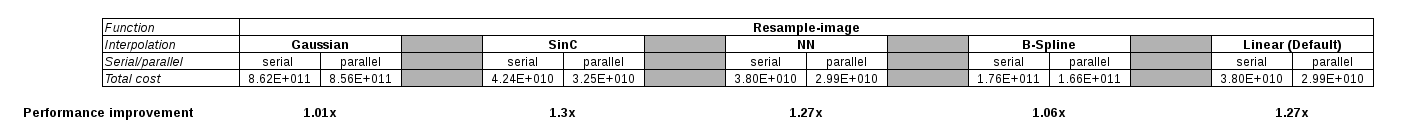
\includegraphics[width=19cm]{figures/tbb_perf_resample-image.png}
	\end{flushleft}	
	\caption{Profilage de resample-image}
	\label{Profilage de resample-image}
\end{figure}
\\
Plusieurs tests ont été lancés sur plusieurs jours concernant la fonction "register" de MIRTK. Les tests sont très longs (15 heures minimum), et les données collectées seront mis en forme la semaine prochaine.
\chapter*{Implémentation}	
Après l'analyse d'une fonction de MIRTK, on doit maintenant passer d'un "Array of Structures" à une "Structure of Arrays".
\paragraph{Stratégie}
Dans un premier temps il s'agit, à partir du profilage effectué, de repérer une fonction de filtrage dont l'implémentation liée à l'éxecution parallèle du programme est relativement simple, afin de se familiariser avec la méthode à employer pour incorporer Arrayfire dans MIRTK.
Ce travailx servira par la suite d'exemple pour plusieurs autres situations car les fonctions dont l'implémentation doit être modifiée utilisent toujours les mêmes modèles de parallélisation (exemple: pour des accumulations, ou des produits matriciels, facilement implémentables avec Arrayfire).
\paragraph{Résultats}
En analysant les données de performances collectées au cours du profiling, on a pu cibler une fonction de filtrage (un floutage, dans ce cas) qui utilise une implémentation plutôt simple à modifier avec ArrayFire, appelée "\textit{smooth-image}"
\newline
- 2 grandes parties dans smooth-image : \\
		\t * Initialisation du kernel\\
		\t => l'implémentation peut se faire complétement en ArrayFire, en se basant sur le travail déjà implémenté dans MIRTK (et peut-être aussi d'ArrayFire en 2D, cf rubrique problèmes)\\
		\newline
			\t * Run\\
			\t 3 étapes : copie du tableau d'entrée, multiplication matricielle, puis  renvoi du tableau de sortie ainsi créé.\\
=> la première étape se fera via une conversion à l'aide d'un contructeur template AF à partir d'un pointeur en paramètre.\\
=> la 2e étape, qui se résume au final à une convolution de matrices, pourra utiliser uniquement des fonctions de ArrayFire, qui sont déjà vectorisées\\
=> la dernière étape se fera grâce à un cast suite à l'étape précedente.\\
		

\paragraph{Problèmes}
- Arrayfire ne dispose pas de kernel (filtre) gaussien en 3 dimensions, mais seulement en 2 dimensions...

\chapter*{Bazar}
\paragraph{Résultats}
Pour transform-image, voici la signature de l'implémentation ArrayFire:
\begin{figure}[h!]
	\begin{center}
		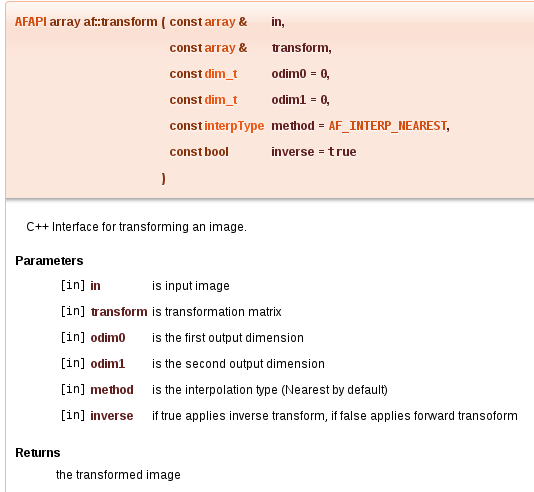
\includegraphics[height=8cm]{figures/transform_af.png}
	\end{center}	
	\caption{Transform-image}
	\label{Transform-image}
\end{figure}
\newline

La variable "method" peut prendre 5 valeurs, correspondant à des interpolations différentes : NN, bilineaire, et indexation par la valeur la plus faible. Aucune de ces types d'interpolations n'est en commun avec celles de MIRTK (exceptée NN), ce qui pourrait éventuellement ajouter des options supplémentaires à MIRTK au futur.
\\
\\
Ci-dessous, on peut voir une image issue de la documentation d'ArrayFire, indiquant les types d'opérations de traitement d'image qui sont implémentées dans ArrayFire.
\begin{figure}[h!]
	\begin{center}
		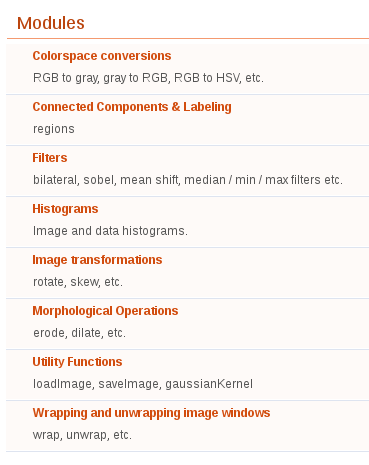
\includegraphics[height=8cm]{figures/list_functions.png}
	\end{center}	
	\caption{Liste des fonctions d'ArrayFire en image processing}
	\label{Liste des fonctions d'ArrayFire en image processing}
\end{figure}
\end{document}